\documentclass[8pt]{article}

\usepackage{../sbc-template} 
\usepackage{graphicx}
\usepackage[utf8]{inputenc} 
\usepackage[T1]{fontenc}
\usepackage[brazil]{babel}
\usepackage[normalem]{ulem}
\usepackage[hidelinks]{hyperref}


\usepackage[square,authoryear]{natbib}
\usepackage{amssymb} 
\usepackage{mathalfa} 
\usepackage{algorithm} 
\usepackage{algpseudocode} 
\usepackage[table]{xcolor}
\usepackage{array}
\usepackage{titlesec}
\usepackage{mdframed}
\usepackage{listings}


\usepackage{amsmath} 
\usepackage{booktabs}
\usepackage[american]{circuitikz}

\urlstyle{same}


\newcolumntype{L}[1]{>{\raggedright\let\newline\\\arraybackslash\hspace{0pt}}m{#1}}
\newcolumntype{C}[1]{>{\centering\let\newline\\\arraybackslash\hspace{0pt}}m{#1}}
\newcolumntype{R}[1]{>{\raggedleft\let\newline\\\arraybackslash\hspace{0pt}}m{#1}}

\newcommand\Tstrut{\rule{0pt}{2.6ex}} 
\newcommand\Bstrut{\rule[-0.9ex]{0pt}{0pt}} 
\newcommand{\scell}[2][c]{\begin{tabular}[#1]{@{}c@{}}#2\end{tabular}}

\usepackage[nolist,nohyperlinks]{acronym}


\title{Finite Element Analysis of Static Systems}

\begin{document} 

% Cover Page
\begin{titlepage}
    \begin{center}
        \vspace*{1cm}
        
        {\Large \textbf{MTE 204 – Numerical Methods}}\\[0.5cm]
        {\Large \textbf{Project 2}}\\[1.5cm]
        
        {\large \textbf{Due Date: Thursday November 28, 2024, 11:59pm}}\\[2cm]
        
        {\large \textbf{Jacob Wielowieyski: 21004619 \& Yarema Dzulynsky: 21014161 }}\\[0.5cm]
        % {\large \textbf{}}\\[3cm]
        
        % Include your university logo in the line below. Replace 'university_logo.png' with the path to your logo file.
        % \includegraphics[width=0.3\textwidth]{university_logo.png}\\[0.5cm]
        
        {\large Instructor: Homeyra Pourmohammadali}\\[0.5cm]
        % {\large MTE 203 - Fall 2024}
        
        \vfill
    \end{center}
\end{titlepage}


\section{Problem 1}
\label{sec:Problem 1}

\subsection{Matrix Equations}
\[
F_i = [k] \times x_i = 
\begin{bmatrix}
    k_i & -k_i \\
    -k_i & k_i
\end{bmatrix}
\times x_i
\]
The k matrix in this problem is given by the stiffness of each spring. Thus, the element matrix equations for this problem are:
\[
\mbox{Spring 1}= 
\begin{bmatrix}
    0.25 & -0.25 \\
    -0.25 & 0.25
\end{bmatrix}
\quad \quad
\mbox{Spring 2}=
\begin{bmatrix}
    0.5 & -0.5 \\
    -0.5 & 0.5
\end{bmatrix}
\quad \quad
\mbox{Spring 3}=
\begin{bmatrix}
    1.5 & -1.5 \\
    -1.5 & 1.5
\end{bmatrix}
\]
\[
\mbox{Spring 4}=
\begin{bmatrix}
    0.75 & -0.75 \\
    -0.75 & 0.75
\end{bmatrix}
\quad \quad
\mbox{Spring 5}=
\begin{bmatrix}
    1 & -1 \\
    -1 & 1
\end{bmatrix}
\]
Combining all of the above equations to create a system, we get the following global assembled matrix equations.
\[
    \begin{bmatrix}
        F_1 \\
        0 \\
        0 \\
        0 \\
        0 \\
        2 \\
    \end{bmatrix}
    =
    \begin{bmatrix}
        0.25 & -0.25 & 0 & 0 & 0 & 0 \\
        -0.25 & 0.25 + 0.5 & -0.5 & 0 & 0 & 0 \\
        0 & -0.5 & 0.5 + 1.5 & -1.5 & 0 & 0 \\
        0 & 0 & -1.5 & 1.5 + 0.75 & -0.75 & 0 \\
        0 & 0 & 0 & -0.75 & 0.75 + 1 & -1 \\
        0 & 0 & 0 & 0 & -1 & 1 \\
    \end{bmatrix}
    \cdot
    \begin{bmatrix}
        x_1 \\
        x_2 \\
        x_3 \\
        x_4 \\
        x_5 \\
        x_6 \\
    \end{bmatrix}
\]
Because \(x_1 = 0\), we can simplify this system into:
\[
\begin{bmatrix} 
    0 \\
    0 \\
    0 \\
    0 \\
    2 \\
\end{bmatrix}
=
\begin{bmatrix}
    0.25 + 0.5 & -0.5 & 0 & 0 & 0 \\
    -0.5 & 0.5 + 1.5 & -1.5 & 0 & 0 \\
    0 & -1.5 & 1.5 + 0.75 & -0.75 & 0 \\
    0 & 0 & -0.75 & 0.75 + 1 & -1 \\
    0 & 0 & 0 & -1 & 1 \\
\end{bmatrix}
\cdot
\begin{bmatrix}
    x_2 \\
    x_3 \\
    x_4 \\
    x_5 \\
    x_6 \\
\end{bmatrix}
\]

\subsection{Problem 1 Answers}
Solving this system with MATLAB, we get the following results. The node displacements (given by the x vector) for each node are:
\[
\begin{bmatrix}
    x_1 \\
    x_2 \\
    x_3 \\
    x_4 \\
    x_5 \\
    x_6 
\end{bmatrix}
=
\begin{bmatrix}
    0 \\
    8 \\
    12 \\
    \frac{40}{3} \\
    16 \\
    18 
\end{bmatrix}
m
\]
The displacement at the final node is given by \(x_6 = 18\)m.
The displacement vs position plot for all the nodes is given in figure~\ref{fig:P1_out}.

\begin{figure}[h!]
    \centering
    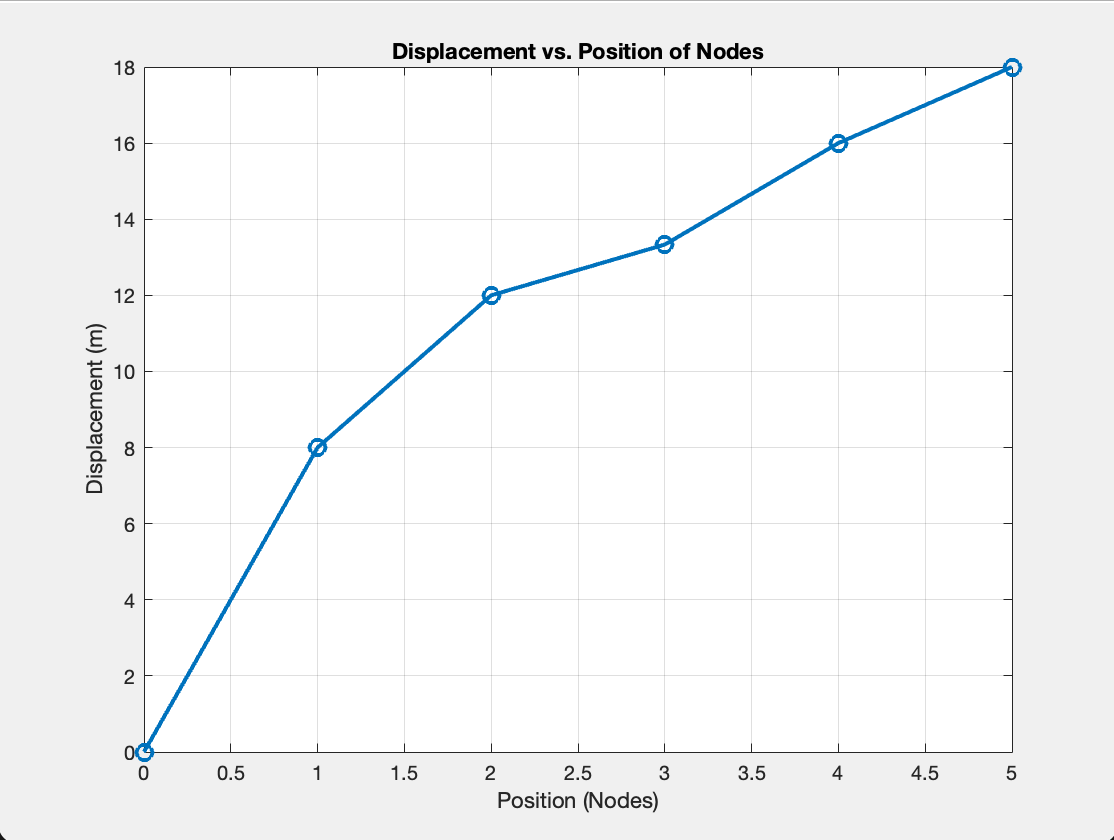
\includegraphics[width=0.5\textwidth]{../../assets/Q1_Graph}
    \caption{Displacement vs Position Plot of Each Node - P1}
    \label{fig:P1_out}
\end{figure}
\break

\section{Problem 2}

\subsection{Matrix Equations}
The k matrix in this problem is derived from the following equation.
\[
\delta = \frac{PL}{EA}
\]
Delta is the displacement, so we will call it x. P is our force. Thus, the remaining components--representing stiffness--are k. Therefore, the element matrix equations for this problem are:
\[
\mbox{Cylinder 1} = 10^9 \cdot
\begin{bmatrix}
    1.4632 & -1.4632 \\
    -1.4632 & 1.4632
\end{bmatrix}
\quad \quad
\mbox{Cylinder 2} = 10^9 \cdot
\begin{bmatrix}
    0.4335 & -0.4335 \\
    -0.4335 & 0.4335
\end{bmatrix}
\]
\[
\mbox{Cylinder 3} = 10^9 \cdot
\begin{bmatrix}
    0.0813 & -0.0813 \\
    -0.0813 & 0.0813
\end{bmatrix}
\]
Combining all of the above equations to create a system, we get the following global assembled matrix equations.
\[
    \begin{bmatrix}
        F_1 \\
        0 \\
        0 \\
        1000
    \end{bmatrix}
    =
    10^9 \cdot
    \begin{bmatrix}
        1.4632 & -1.4632 & 0 & 0 \\
        -1.4632 & 1.8967 & -0.4335 & 0 \\
         0 & -0.4335 & 0.5148 & -0.0813 \\
         0 & 0 & -0.0813 & 0.0813
    \end{bmatrix}
    \cdot
    \begin{bmatrix}
        x_1 \\
        x_2 \\
        x_3 \\
        x_4 \\
    \end{bmatrix}
\]
Because \(x_1 = 0\), we can simplify this system into:
\[
\begin{bmatrix}
    0 \\ 
    0 \\ 
    1000 \\
\end{bmatrix}
=
10^9 \cdot
\begin{bmatrix}
    1.897 & -0.4335 & 0 \\
    -0.4335 & 0.5148 & -0.0813 \\
    0 & -0.0813 & -0.0813\\
\end{bmatrix}
\cdot
\begin{bmatrix}
    x_2 \\ 
    x_3 \\ 
    x_4 \\
\end{bmatrix}
\]

\subsection{Problem 2 Answers}
Solving this system with MATLAB, we get the following results. The node displacements (given by the x vector) for each node are:
\[
\begin{bmatrix}
    x_1 \\
    x_2 \\
    x_3 \\
    x_4 
\end{bmatrix}
=
10^{-5} \cdot
\begin{bmatrix}
    0 \\
    0.0683 \\
    0.299 \\
    1.5292 
\end{bmatrix}
m
\]
The displacement at the final node is given by \(x_4 = 10^{-5}\cdot1.5292\)m.
The displacement vs position plot for all the nodes is given in figure~\ref{fig:P2_out}.
\begin{figure}[h!]
    \centering
    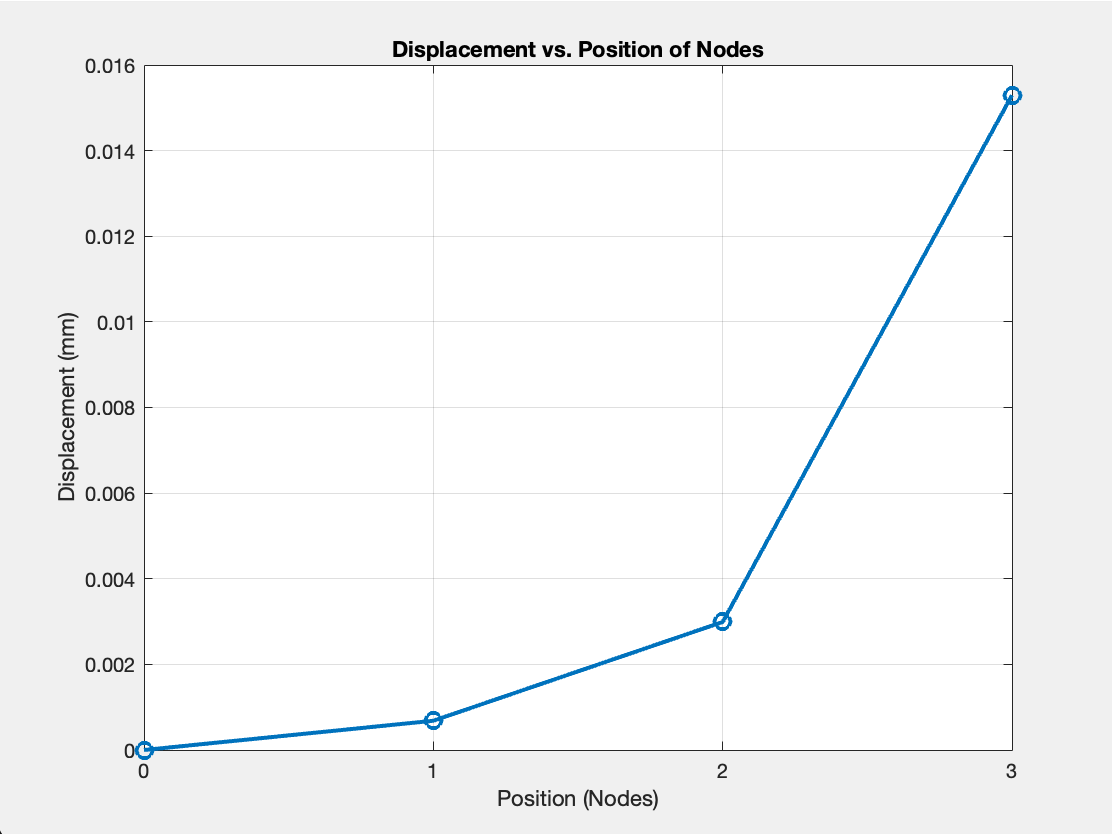
\includegraphics[width=0.5\textwidth]{../../assets/Q2_Graph}
    \caption{Displacement vs Position Plot of Each Node - P2}
    \label{fig:P2_out}
\end{figure}



\section{Problem 3}

\subsection{Matrix Equations}
Much as in problem 2, the k value for this problem is given by \(k=\frac{AE}{L}\). The k matrix must now account for the additional dimension, thus the general stiffness matrix is given by:
\[
k=\frac{AE}{L}
\begin{bmatrix}
    \cos\theta^2 & \cos\theta\sin\theta & -\cos\theta^2 & -\cos\theta\sin\theta \\
    \cos\theta\sin\theta & \sin\theta^2 & -\cos\theta\sin\theta & -\sin\theta^2 \\
    -\cos\theta^2 & -\cos\theta\sin\theta & \cos\theta^2 & \cos\theta\sin\theta \\
    -\cos\theta\sin\theta & -\sin\theta^2 & \cos\theta\sin\theta & \sin\theta^2 \\
\end{bmatrix}
\]
Thus, the element matrix equations for this problem are:
\[
k_1 = 10^7 \times
\begin{bmatrix}
1.6667 & 2.8868 & -1.6667 & -2.8868 & 0 & 0 & 0 & 0 & 0 & 0 \\
2.8868 & 5.0000 & -2.8868 & -5.0000 & 0 & 0 & 0 & 0 & 0 & 0 \\
-1.6667 & -2.8868 & 1.6667 & 2.8868 & 0 & 0 & 0 & 0 & 0 & 0 \\
-2.8868 & -5.0000 & 2.8868 & 5.0000 & 0 & 0 & 0 & 0 & 0 & 0 \\
0 & 0 & 0 & 0 & 0 & 0 & 0 & 0 & 0 & 0 \\
0 & 0 & 0 & 0 & 0 & 0 & 0 & 0 & 0 & 0 \\
0 & 0 & 0 & 0 & 0 & 0 & 0 & 0 & 0 & 0 \\
0 & 0 & 0 & 0 & 0 & 0 & 0 & 0 & 0 & 0 \\
0 & 0 & 0 & 0 & 0 & 0 & 0 & 0 & 0 & 0 \\
0 & 0 & 0 & 0 & 0 & 0 & 0 & 0 & 0 & 0 \\
\end{bmatrix}
\]

\[
k_2 = 10^7 \times
\begin{bmatrix}
6.6667 & 0 & 0 & 0 & -6.6667 & 0 & 0 & 0 & 0 & 0 \\
0 & 0 & 0 & 0 & 0 & 0 & 0 & 0 & 0 & 0 \\
0 & 0 & 0 & 0 & 0 & 0 & 0 & 0 & 0 & 0 \\
0 & 0 & 0 & 0 & 0 & 0 & 0 & 0 & 0 & 0 \\
-6.6667 & 0 & 0 & 0 & 6.6667 & 0 & 0 & 0 & 0 & 0 \\
0 & 0 & 0 & 0 & 0 & 0 & 0 & 0 & 0 & 0 \\
0 & 0 & 0 & 0 & 0 & 0 & 0 & 0 & 0 & 0 \\
0 & 0 & 0 & 0 & 0 & 0 & 0 & 0 & 0 & 0 \\
0 & 0 & 0 & 0 & 0 & 0 & 0 & 0 & 0 & 0 \\
0 & 0 & 0 & 0 & 0 & 0 & 0 & 0 & 0 & 0 \\
\end{bmatrix}
\]

\[
k_3 = 10^7 \times
\begin{bmatrix}
0 & 0 & 0 & 0 & 0 & 0 & 0 & 0 & 0 & 0 \\
0 & 0 & 0 & 0 & 0 & 0 & 0 & 0 & 0 & 0 \\
0 & 0 & 1.6667 & -2.8868 & -1.6667 & 2.8868 & 0 & 0 & 0 & 0 \\
0 & 0 & -2.8868 & 5.0000 & 2.8868 & -5.0000 & 0 & 0 & 0 & 0 \\
0 & 0 & -1.6667 & 2.8868 & 1.6667 & -2.8868 & 0 & 0 & 0 & 0 \\
0 & 0 & 2.8868 & -5.0000 & -2.8868 & 5.0000 & 0 & 0 & 0 & 0 \\
0 & 0 & 0 & 0 & 0 & 0 & 0 & 0 & 0 & 0 \\
0 & 0 & 0 & 0 & 0 & 0 & 0 & 0 & 0 & 0 \\
0 & 0 & 0 & 0 & 0 & 0 & 0 & 0 & 0 & 0 \\
0 & 0 & 0 & 0 & 0 & 0 & 0 & 0 & 0 & 0 \\
\end{bmatrix}
\]

\[
k_4 = 10^7 \times
\begin{bmatrix}
0 & 0 & 0 & 0 & 0 & 0 & 0 & 0 & 0 & 0 \\
0 & 0 & 0 & 0 & 0 & 0 & 0 & 0 & 0 & 0 \\
0 & 0 & 0 & 0 & 0 & 0 & 0 & 0 & 0 & 0 \\
0 & 0 & 0 & 0 & 0 & 0 & 0 & 0 & 0 & 0 \\
0 & 0 & 0 & 0 & 1.6667 & 2.8868 & -1.6667 & -2.8868 & 0 & 0 \\
0 & 0 & 0 & 0 & 2.8868 & 5.0000 & -2.8868 & -5.0000 & 0 & 0 \\
0 & 0 & 0 & 0 & -1.6667 & -2.8868 & 1.6667 & 2.8868 & 0 & 0 \\
0 & 0 & 0 & 0 & -2.8868 & -5.0000 & 2.8868 & 5.0000 & 0 & 0 \\
0 & 0 & 0 & 0 & 0 & 0 & 0 & 0 & 0 & 0 \\
0 & 0 & 0 & 0 & 0 & 0 & 0 & 0 & 0 & 0 \\
\end{bmatrix}
\]

\[
k_5 = 10^7 \times
\begin{bmatrix}
0 & 0 & 0 & 0 & 0 & 0 & 0 & 0 & 0 & 0 \\
0 & 0 & 0 & 0 & 0 & 0 & 0 & 0 & 0 & 0 \\
0 & 0 & 0 & 0 & 0 & 0 & 0 & 0 & 0 & 0 \\
0 & 0 & 0 & 0 & 0 & 0 & 0 & 0 & 0 & 0 \\
0 & 0 & 0 & 0 & 6.6667 & 0 & 0 & 0 & -6.6667 & 0 \\
0 & 0 & 0 & 0 & 0 & 0 & 0 & 0 & 0 & 0 \\
0 & 0 & 0 & 0 & 0 & 0 & 0 & 0 & 0 & 0 \\
0 & 0 & 0 & 0 & 0 & 0 & 0 & 0 & 0 & 0 \\
0 & 0 & 0 & 0 & -6.6667 & 0 & 0 & 0 & 6.6667 & 0 \\
0 & 0 & 0 & 0 & 0 & 0 & 0 & 0 & 0 & 0 \\
\end{bmatrix}
\]

\[
k_6 = 10^7 \times
\begin{bmatrix}
0 & 0 & 0 & 0 & 0 & 0 & 0 & 0 & 0 & 0 \\
0 & 0 & 0 & 0 & 0 & 0 & 0 & 0 & 0 & 0 \\
0 & 0 & 0 & 0 & 0 & 0 & 0 & 0 & 0 & 0 \\
0 & 0 & 0 & 0 & 0 & 0 & 0 & 0 & 0 & 0 \\
0 & 0 & 0 & 0 & 0 & 0 & 0 & 0 & 0 & 0 \\
0 & 0 & 0 & 0 & 0 & 0 & 0 & 0 & 0 & 0 \\
0 & 0 & 0 & 0 & 0 & 0 & 1.6667 & -2.8868 & -1.6667 & 2.8868 \\
0 & 0 & 0 & 0 & 0 & 0 & -2.8868 & 5.0000 & 2.8868 & -5.0000 \\
0 & 0 & 0 & 0 & 0 & 0 & -1.6667 & 2.8868 & 1.6667 & -2.8868 \\
0 & 0 & 0 & 0 & 0 & 0 & 2.8868 & -5.0000 & -2.8868 & 5.0000 \\
\end{bmatrix}
\]

\[
k_7 = 10^7 \times
\begin{bmatrix}
0 & 0 & 0 & 0 & 0 & 0 & 0 & 0 & 0 & 0 \\
0 & 0 & 0 & 0 & 0 & 0 & 0 & 0 & 0 & 0 \\
0 & 0 & 6.6667 & 0 & 0 & 0 & -6.6667 & 0 & 0 & 0 \\
0 & 0 & 0 & 0 & 0 & 0 & 0 & 0 & 0 & 0 \\
0 & 0 & 0 & 0 & 0 & 0 & 0 & 0 & 0 & 0 \\
0 & 0 & 0 & 0 & 0 & 0 & 0 & 0 & 0 & 0 \\
0 & 0 & -6.6667 & 0 & 0 & 0 & 6.6667 & 0 & 0 & 0 \\
0 & 0 & 0 & 0 & 0 & 0 & 0 & 0 & 0 & 0 \\
0 & 0 & 0 & 0 & 0 & 0 & 0 & 0 & 0 & 0 \\
0 & 0 & 0 & 0 & 0 & 0 & 0 & 0 & 0 & 0 \\
\end{bmatrix}
\]
Combining all of the above equations to create a system, we get the following global assembled stiffness matrix.
\[
10^8 \cdot
\begin{bmatrix}
    0.8333 & 0.2887 & -0.1667 & -0.2887 & -0.6667 & 0 & 0 & 0 & 0 & 0 \\
    0.2887 & 0.5 & -0.2887 & -0.5 & 0 & 0 & 0 & 0 & 0 & 0 \\
    -0.1667 & -0.2887 & 1 & 0 & -0.1667 & 0.2887 & -0.6667 & 0 & 0 & 0 \\
    -0.2887 & -0.5 & 0 & 1 & 0.2887 & -0.5 & 0 & 0 & 0 & 0 \\
    -0.6667 & 0 & -0.1667 & 0.2887 & 1.6667 & 0 & -0.1667 & -0.2887 & -0.6667 & 0 \\
    0 & 0 & 0.2887 & -0.5 & 0 & 1 & -0.2887 & -0.5 & 0 & 0 \\
    0 & 0 & -0.6667 & 0 & -0.1667 & -0.2887 & 1 & 0 & -0.1667 & 0.2887 \\
    0 & 0 & 0 & 0 & -0.2887 & -0 & 0 & 1.0000 & 0.2887 & -0.5 \\
    0 & 0 & 0 & 0 & -0.6667 & 0 & -0.1667 & 0.2887 & 0.8333 & -0.2887 \\
    0 & 0 & 0 & 0 & 0 & 0 & 0.2887 & -0.5 & -0.2887 & 0.5
\end{bmatrix}
\]
Recognizing that y is constrained at nodes 1 and 5 by the roller, we get the following simplified equation by removing rows and columns 2 and 10, corresponding to \(x_2\) and \(x_{10}\), which must be 0 as displacement is 0.
\[
\begin{bmatrix}
    0 \\
    0 \\
    -2000 \\
    0 \\
    0 \\
    0 \\
    -5000 \\
    0 \\
\end{bmatrix}
=
10^8 \times
\begin{bmatrix}
    0.833 & -0.167 & -0.289 & -0.667 & 0 & 0 & 0 & 0 \\
    -0.167 & 1 & 0 & -0.167 & 0.289 & -0.667 & 0 & 0 \\
    -0.289 & 0 & 1 & 0.289 & -0.5 & 0 & 0 & 0 \\
    -0.667 & -0.167 & 0.289 & 1.667 & 0 & -0.167 & -0.289 & -0.667 \\
    0 & 0.289 & -0.5 & 0 & 1 & -0.289 & -0.5 & 0 \\
    0 & -0.667 & 0 & -0.167 & -0.289 & 1 & 0 & -0.167 \\
    0 & 0 & 0 & -0.289 & -0.5 & 0 & 1 & 0.289 \\
    0 & 0 & 0 & -0.667 & 0 & -0.167 & 0.289 & 0.833 \\
\end{bmatrix}
\times
\begin{bmatrix}
    x_1 \\
    % x_2 \\
    x_3 \\
    x_4 \\
    x_5 \\
    x_6 \\
    x_7 \\
    x_8 \\
    x_9 \\
\end{bmatrix}
\]

\subsection{Problem 3 Answers}
Solving this system with MATLAB, we get the following results. The global node displacements (given by the x vector)for each node are:
\[
    \text{Displacement} = 10^{-3} \times 
    \begin{bmatrix}
        -0.0242 \\
        0 \\
        0.0180 \\
        -0.0794 \\
        -0.0004 \\
        -0.1050 \\
        -0.0123 \\
        -0.1131 \\
        0.0364 \\
        0 \\
    \end{bmatrix}
    \text{m}
\]
The normal stresses in each member are:
\[
    \text{Normal Stresses in Each Member} =
    \begin{bmatrix}
        -7.939 \\
        3.969 \\
        2.165 \\
        -2.165 \\
        6.134 \\
        -12.269 \\
        -5.052 \\
    \end{bmatrix}
    \text{MPa}
\]
The x and y components of displacement for each node is:
\[
\text{x component} = 10^{-5} \times
\begin{bmatrix}
    -2.419 \\
    1.803 \\
    -0.03693 \\
    -1.228 \\
    3.644
\end{bmatrix} \text{ m}
\]

\[
\text{y component} = 10^{-5} \times
\begin{bmatrix}
    0 \\
    -7.938 \\
    -10.50 \\
    -11.31 \\
    0
\end{bmatrix} \text{ m}
\]

\end{document}